%!TEX TS-program = xelatex
%!TEX encoding = UTF-8 Unicode

% \documentclass{article} % For LaTeX2e
% \usepackage{nips,times}
% \usepackage{hyperref}
% \usepackage{url}
% %\documentstyle[nips14submit_09,times,art10]{article} % For LaTeX 2.09


% \title{Proposal for sparse PCA in financial series}


% \author{
% Chengzhe Yan\\
% %\thanks{ Use footnote for providing further information about author (webpage, alternative address)---\emph{not} for acknowledging funding agencies.} \\
% Department of Automation\\
% Tsinghua University\\
% Beijing, 15213 \\
% \texttt{yancz12@mails.tsinghua.edu.cn} \\
% }

% % The \author macro works with any number of authors. There are two commands
% % used to separate the names and addresses of multiple authors: \And and \AND.
% %
% % Using \And between authors leaves it to \LaTeX{} to determine where to break
% % the lines. Using \AND forces a linebreak at that point. So, if \LaTeX{}
% % puts 3 of 4 authors names on the first line, and the last on the second
% % line, try using \AND instead of \And before the third author name.

% \newcommand{\fix}{\marginpar{FIX}}
% \newcommand{\new}{\marginpar{NEW}}

%\nipsfinalcopy % Uncomment for camera-ready version
%
% This is the LaTeX template file for lecture notes for CS267,
% Applications of Parallel Computing.  When preparing
% LaTeX notes for this class, please use this template.
%
% To familiarize yourself with this template, the body contains
% some examples of its use.  Look them over.  Then you can
% run LaTeX on this file.  After you have LaTeXed this file then
% you can look over the result either by printing it out with
% dvips or using xdvi.
%

\documentclass[oneside]{article}
%
% ADD PACKAGES here:
%

\usepackage{amsfonts}
\usepackage{indentfirst}
\usepackage{amsmath}
\usepackage{amssymb}
\usepackage{multirow}
\usepackage{array}  
\usepackage{algorithm2e}
\usepackage{xeCJK}    
\usepackage{longtable}
\usepackage{graphicx}
\usepackage{subfigure}
\usepackage{geometry}
\usepackage{color}
\usepackage{url}
\usepackage{fancyhdr}
\usepackage{enumitem}
\usepackage{parskip}

\setlength{\oddsidemargin}{0 in}
\setlength{\evensidemargin}{0 in}
\setlength{\topmargin}{-0.6 in}
\setlength{\textwidth}{6.5 in}
\setlength{\textheight}{8.5 in}
\setlength{\headsep}{0.75 in}
\setlength{\parindent}{0 in}
\setlength{\parskip}{5pt}
\setlist[itemize]{parsep=0pt}
\setlist[enumerate]{parsep=0pt}
\linespread{1.4}
\geometry{a4paper}

\usepackage{fontspec,indentfirst}

\setCJKfamilyfont{kaiti}{Kaiti SC Regular}
\newcommand*{\kai}{\CJKfamily{kaiti}} % 楷体_GB2312
\setCJKfamilyfont{heiti}{Heiti SC Light}
\newcommand*{\hei}{\CJKfamily{heiti}} % 黑体
\setCJKfamilyfont{song}{Songti SC Regular}  
\newcommand*{\song}{\CJKfamily{song}} % 宋体
\setCJKfamilyfont{fangsong}{FangSong}
\newcommand*{\fang}{\CJKfamily{fangsong}}  % 仿宋
\renewcommand \tablename 表{}
\renewcommand \figurename 图{}
\defaultfontfeatures{Mapping=tex-text}  
\setCJKmainfont{Songti SC Regular}

\XeTeXlinebreaklocale "zh"
\XeTeXlinebreakskip=0pt plus 1pt minus 0.1pt

%
% The following commands set up the lecnum (lecture number)
% counter and make various numbering schemes work relative
% to the lecture number.
%
\renewcommand{\thepage}{\arabic{page}}
\renewcommand{\thesection}{\arabic{section}}
\renewcommand{\theequation}{\arabic{section}.\arabic{equation}}
\renewcommand{\thefigure}{\arabic{section}.\arabic{figure}}
\renewcommand{\thetable}{\arabic{section}.\arabic{table}}
\renewcommand{\baselinestretch}{1.4} \normalsize

\DeclareMathOperator*{\argmin}{\arg\!\min}

%
% The following macro is used to generate the header.
\newcommand{\lecture}[5]{
   \newpage
   \noindent
   \begin{center}
        {\LARGE \bf #1} \\
        \vspace{0.5cm}
        {\bf #2} \\
        \vspace{0cm}
        #3\\
        \vspace{0.3cm}
        \it Date: #4
   \end{center}
}
%
% Convention for citations is authors' initials followed by the year.
% For example, to cite a paper by Leighton and Maggs you would type
% \cite{LM89}, and to cite a paper by Strassen you would type \cite{S69}.
% (To avoid bibliography problems, for now we redefine the \cite command.)
% Also commands that create a suitable format for the reference list.
\renewcommand{\cite}[1]{[#1]}
\def\beginrefs{\begin{list}%
        {[\arabic{equation}]}{\usecounter{equation}
         \setlength{\leftmargin}{2.0truecm}\setlength{\labelsep}{0.4truecm}%
         \setlength{\labelwidth}{1.6truecm}}}
\def\endrefs{\end{list}}
\def\bibentry#1{\item[\hbox{[#1]}]}

%Use this command for a figure; it puts a figure in wherever you want it.
%usage: \fig{NUMBER}{SPACE-IN-INCHES}{CAPTION}
\newcommand{\fig}[2]{
            \vspace{#1}
            \begin{center}
            Figure ~#2
            \end{center}
    }
% Use these for theorems, lemmas, proofs, etc.
%
\newcounter{theorem_no}[section]
\newcounter{definition_no}[section]
\newtheorem{theorem}{Theorem}[section]
\newtheorem{lemma}[theorem]{Lemma}
\newtheorem{proposition}[theorem]{Proposition}
\newtheorem{claim}[theorem]{Claim}
\newtheorem{corollary}[theorem]{Corollary}
\newtheorem{definition}[definition_no]{Definition}
\newenvironment{proof}{{\bf Proof:}}{\hfill\rule{2mm}{2mm}}

% **** IF YOU WANT TO DEFINE ADDITIONAL MACROS FOR YOURSELF, PUT THEM HERE:

\newcommand\E{\mathbb{E}}

\begin{document}
\graphicspath{{figures/}}
\lecture{BatchInhib}{Rui Lu}{Bigeye}{Jul. 4 2016}

\section{Inhibition via Mini-Batch Statistics}
在一个$mini-batch$中, 考虑某个$feature\ map$ $\{x_{i}^{(j)}\}$($i = 1, ..., N$表示$feature$的维度,$j = 1, ..., m$表示$batch\ size$), 相互抑制的作用可以表示如下:
\begin{eqnarray}
\mu_{x_{i}} = \frac{1}{m}\sum_{j=1}^{m}x_{i}^{(j)} \\
\sigma_{x_{i}} = \frac{1}{m}\sum_{j=1}^{m}(x_{i}^{(j)} - \mu_{x_{i}})^{2} \\
r_{ik} = \frac{\frac{1}{m}[\sum_{j=1}^{m}(x_{i}^{(j)} - \mu_{x_{i}})(x_{k}^{(j)} - \mu_{x_{k}})]}{\sigma_{x_{i}}\sigma_{x_{k}}} \\
R_{ik} = \frac{g(\alpha_{ik})r_{ik}}{\sum_{l\neq i}g(\alpha_{il})r_{il}} \\
y_{i}^{(j)} = x_{i}^{(j)} - \sum_{l\neq i}R_{il}x_{l}^{(j)}
\end{eqnarray}
其中,$g(x) = \frac{1}{\rho}log(1 + e^{\rho x})$\\
对上面的式子求导:
\begin{eqnarray}
\frac{\partial L}{\partial R_{ik}} = \sum_{j=1}^{m}\frac{\partial L}{\partial y_{i}^{(j)}}\frac{\partial y_{i}^{(j)}}{\partial R_{ik}}=\sum_{j=1}^{m}\frac{\partial L}{\partial y_{i}^{(j)}}(-x_{k}^{(j)}) \\
\frac{\partial L}{\partial \alpha_{ik}} = \frac{\partial L}{\partial R_{ik}}\frac{\partial R_{ik}}{\partial \alpha_{ik}}=\frac{\partial L}{\partial R_{ik}}\frac{r_{ik}[\sum_{l\neq i}g(\alpha_{il})r_{il} - g(\alpha_{ik})r_{ik}]}{[\sum_{l\neq i}g(\alpha_{il})r_{il}]^{2}}g^{\prime}(\alpha_{ik}) \\
\frac{\partial L}{\partial r_{ik}} = \frac{\partial L}{\partial R_{ik}}\frac{\partial R_{ik}}{\partial r_{ik}} = \frac{g(\alpha_{ik})[\sum_{l\neq i}g(\alpha_{il})r_{il} - g(\alpha_{ik})r_{ik}]}{[\sum_{l\neq i}g(\alpha_{il})r_{il}]^{2}} \\
\frac{\partial L}{\partial \sigma_{x_{i}}} = \frac{\partial L}{\partial r_{ik}}\frac{\partial r_{ik}}{\partial \sigma_{x_{i}}}=\frac{(-1)}{\sigma_{x_{i}}^{2}}\frac{\frac{1}{m}[\sum_{j=1}^{m}(x_{i}^{(j)} - \mu_{x_{i}})(x_{k}^{(j)} - \mu_{x_{k}})]}{\sigma_{x_{k}}} \\
\frac{\partial L}{\partial \mu_{x_{i}}} = \frac{\partial L}{\partial r_{ik}}\frac{\partial r_{ik}}{\partial \mu_{x_{i}}} + \frac{\partial L}{\partial \sigma_{x_{i}}}\frac{\partial \sigma_{x_{i}}}{\partial \mu_{x_{i}}} = \nonumber \\
\frac{\partial L}{\partial r_{ik}}\frac{\frac{1}{m}[\sum_{j=1}^{m}(-1)(x_{k}^{(j)} - \mu_{x_{k}})]}{\sigma_{x_{i}}\sigma_{x_{k}}} + \frac{\partial L}{\partial \sigma_{x_{i}}}\frac{(-1)}{2m}\sum_{j=1}^{m}(x_{i}^{(j)} - \mu_{x_{i}}) \\
\frac{\partial L}{\partial x_{i}^{(j)}} = \frac{\partial L}{\partial \mu_{x_{i}}}\frac{\partial \mu_{x_{i}}}{\partial x_{i}^{(j)}} + \frac{\partial L}{\partial \sigma_{x_{i}}}\frac{\partial \sigma_{x_{i}}}{\partial x_{i}^{(j)}} + \frac{\partial L}{\partial r_{ik}}\frac{\partial r_{ik}}{\partial x_{i}^{(j)}} + \frac{\partial L}{\partial y_{i}^{(j)}}\frac{\partial y_{i}^{(j)}}{\partial x_{i}^{(j)}} = \nonumber \\
 \frac{\partial L}{\partial \mu_{x_{i}}}\frac{1}{m}
+ \frac{\partial L}{\partial \sigma_{x_{i}}}\frac{2}{m}(x_{i}^{(j)} - \mu_{x_{i}})
+ \frac{\partial L}{\partial r_{ik}}\frac{1}{m}\frac{(x_{k}^{(j)} - \mu_{x_{k}})}{\sigma_{x_{i}}\sigma_{x_{k}}}
+ \frac{\partial L}{\partial y_{i}^{(j)}} 
\end{eqnarray}

% template for algorithm
%\begin{algorithm}[H]
% \For{t=1...maxIter}{
% $L = L(x_{t}, W, U)$ \\
% $\frac{\partial L}{\partial W} \longrightarrow W_{new}$ \\
% $L = L(x_{t}, W_{new}, U)$ \\
% $\frac{\partial L}{\partial U} \longrightarrow U_{new}$}
% \caption{第一种异步迭代方式,将\textcolor{red}{一次求导拆分为两次}}
%\end{algorithm}
%\vspace{0.5cm}

% template for figure
%\begin{figure}[h]
%\centering
%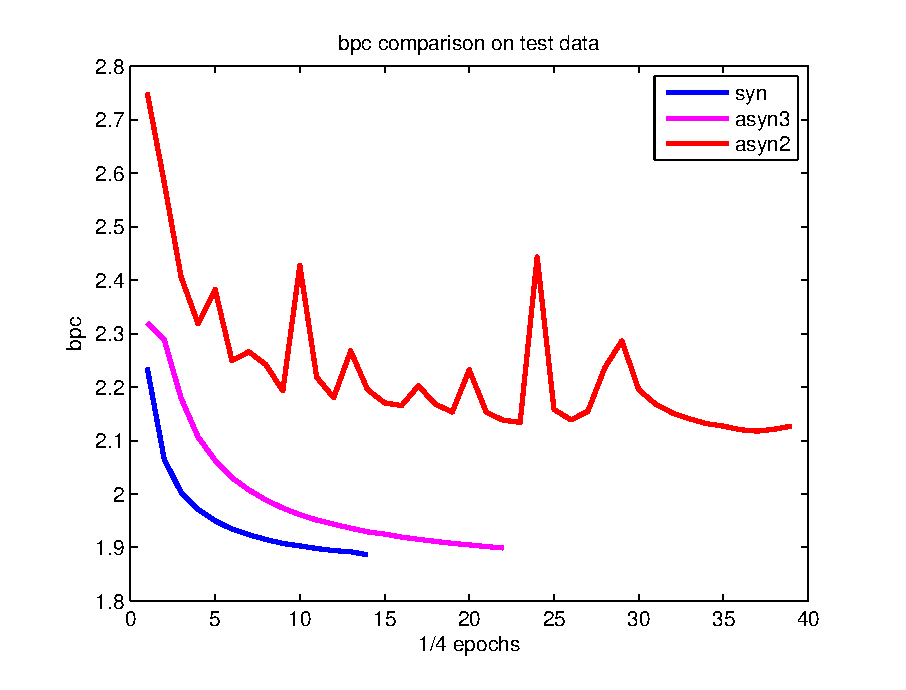
\includegraphics[height=.35\textheight,width=.8\textwidth]{bpc_compare}
%\vspace{-0cm}\caption{bpc与迭代轮数的关系}
%\label{fig:bpc_compare}
%\end{figure}


\end{document}
